\subsection{sbRIO}

The embedded system controlling the EndoWrist contains a \textbf{Single Board Reconfigurable Input/Output 9636} (sbRIO) controller, see \figref{fig:sbRIO9636}. It is responsible for interfacing between the surgical robot and the computer running the robotic operating system\cite{Chris_Surgical}, see \secref{sec:ros}. It reads the data sent by the ESCON drivers, sends them to the PC and position controls the motors based on the received reference signals. The sbRIO has built in safety protocols that disable the motors in case of error.

\begin{figure}[H]
	\centering
		\centering
<		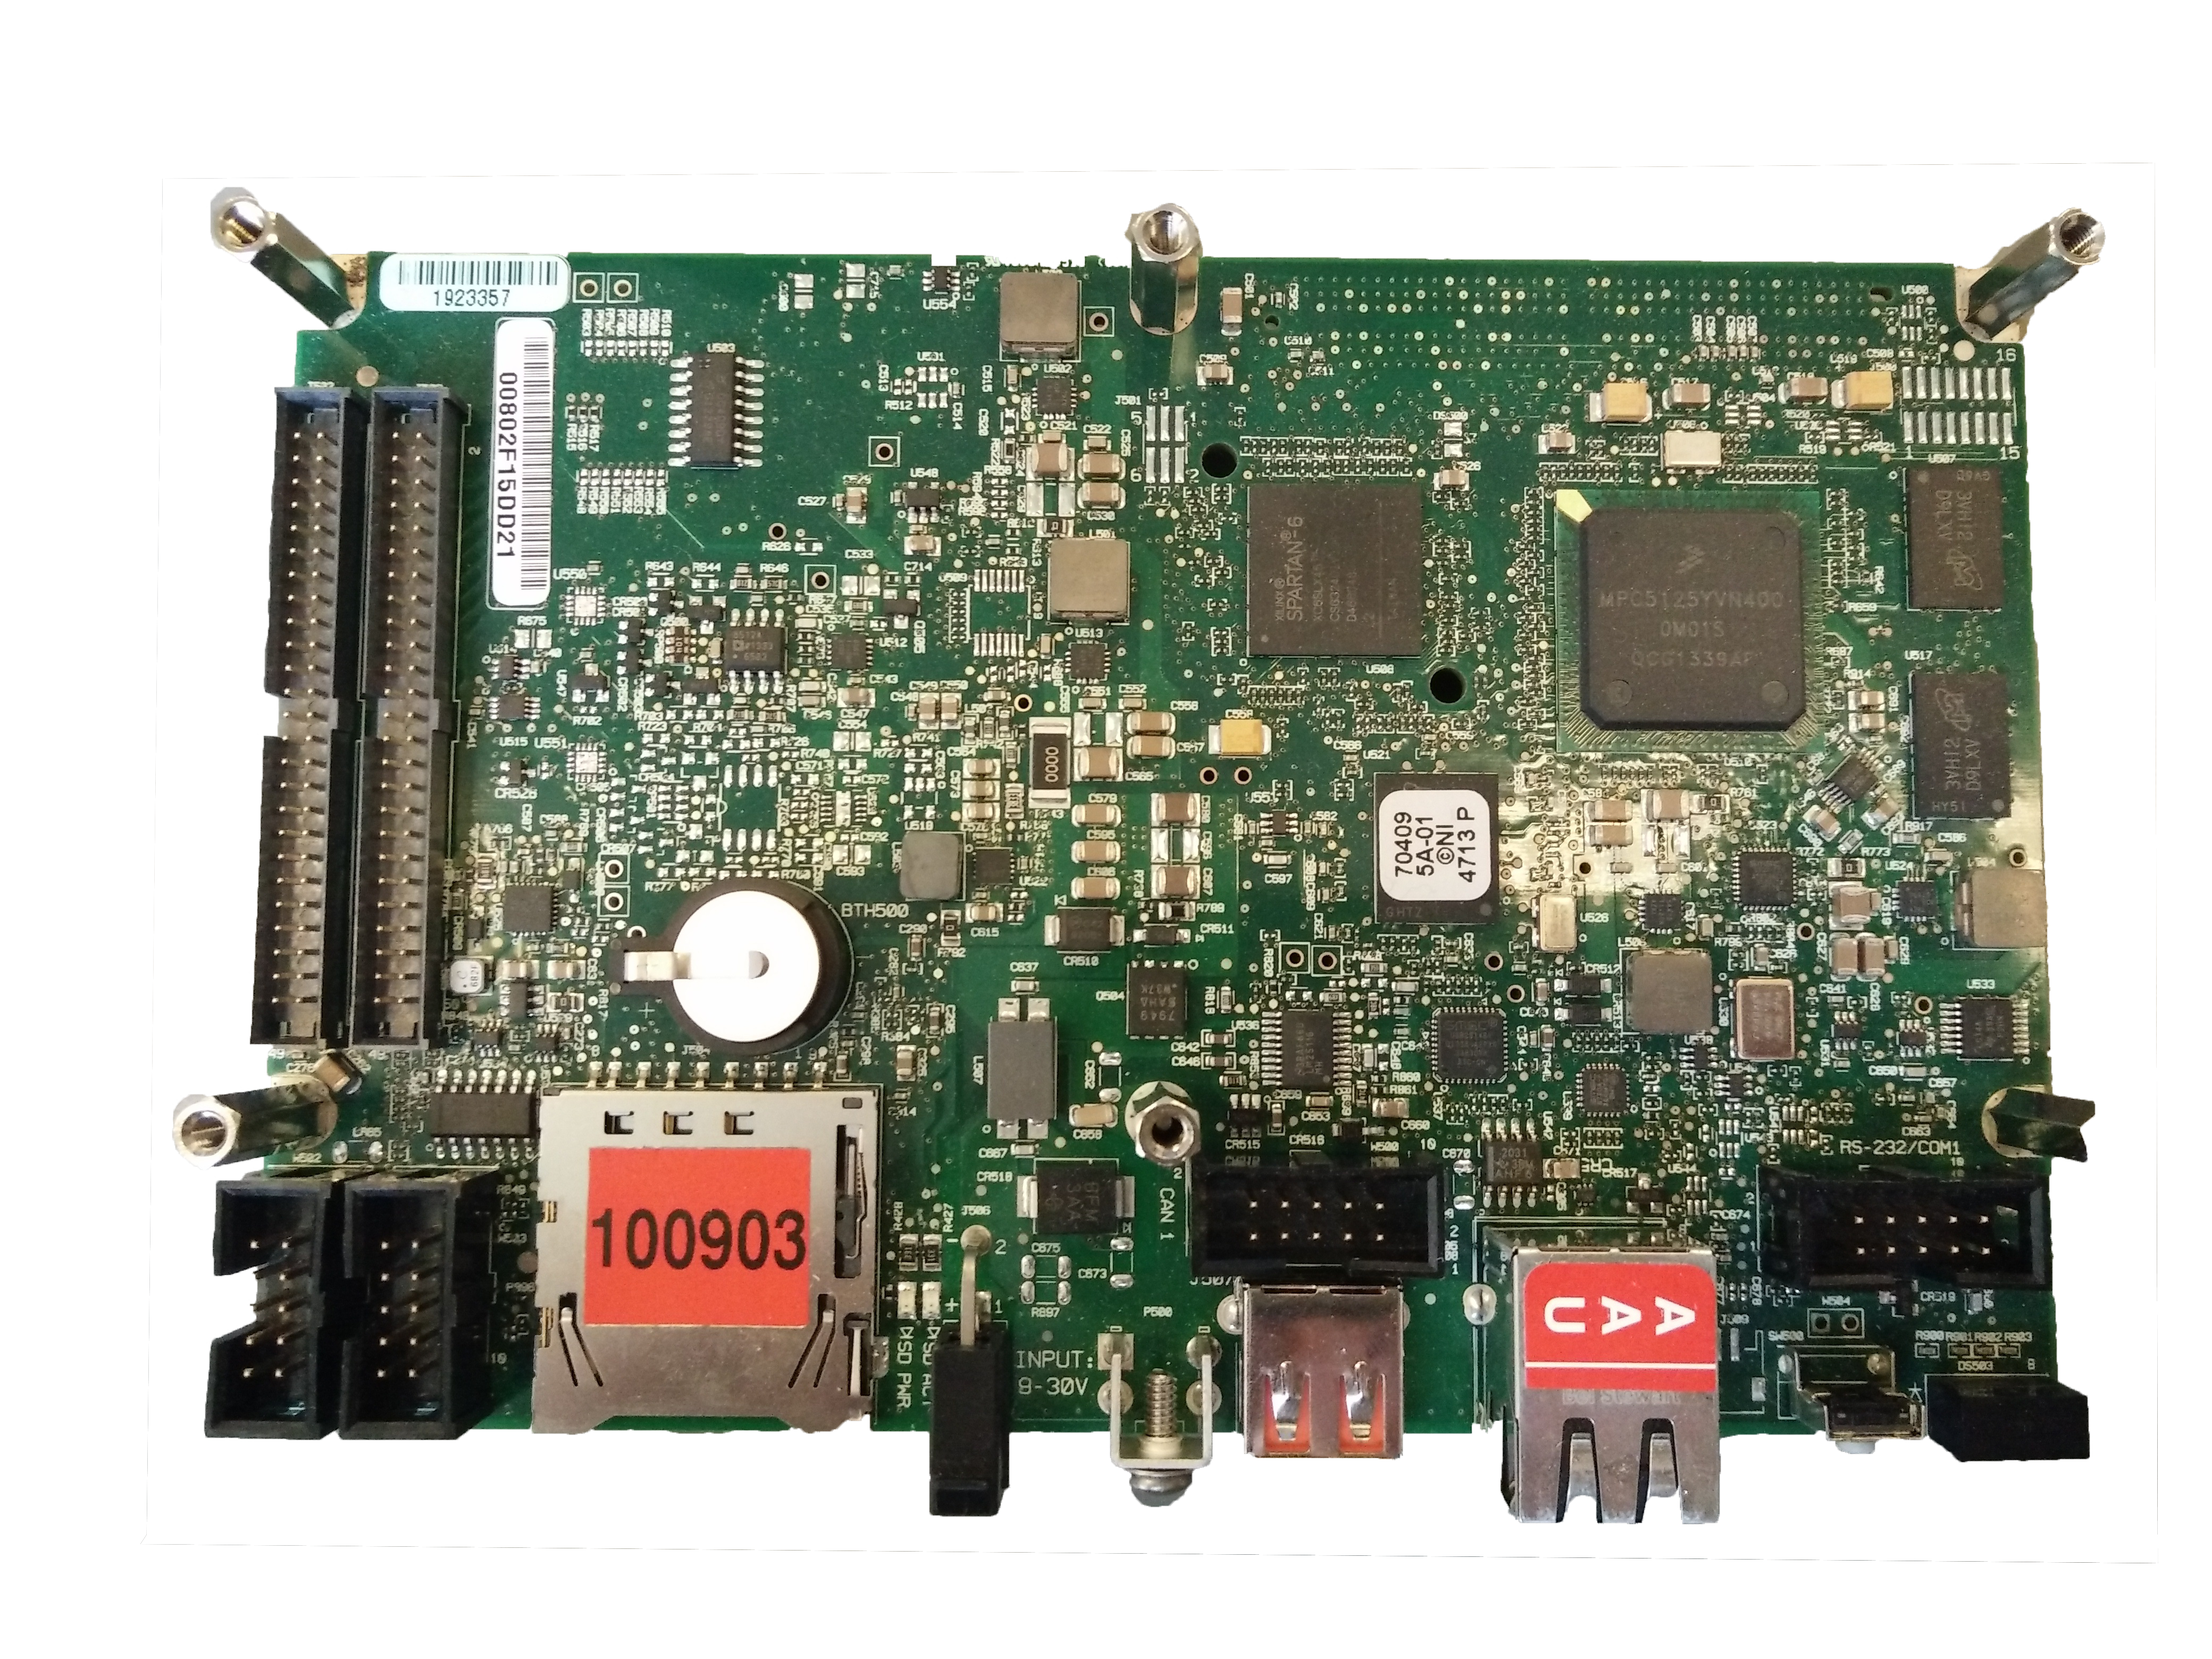
\includegraphics[width=0.7\linewidth]{sbRIO9636.png}
		\caption{The sbRIO 9636 board\cite{sbRIO9636Pic}}
		\label{fig:sbRIO9636}
\end{figure}


The controller consists of
\begin{itemize}
	\item 400 MHz real time processor
	\item 256 MB of system memory and 512 MB nonvolatile memory
	\item Reconfigurable Xilinx Spartan-6 LX45 FPGA
	\item 16 bit analog and digital I/O
	\item Built in USB, CAN, 10/100 Mb/s Ethernet peripherials
\end{itemize}

The board is configured through an ethernet cable. The programs can be written using Labview, C or C++. In the present project, LabView will be used due to the simplicity of coding the FPGA through a high level language. The board is capable of running in real-time. %code, which is unmatched on the ROS side.

% http://sine.ni.com/nips/cds/view/p/lang/en/nid/210421


%\begin{figure}[H]
\begin{tikzpicture}

\node[state] (Endowrist) 
{
	%\parbox[c][2cm][c]{4cm}{\hspace{2.5em} \textbf{Endowrist}}
	\parbox[c][1.5cm][c]{2cm}{\textbf{Endowrist}}
};

\node[state,       % layout (defined above)
node distance=4cm,     
right of=Endowrist,        % Position is to the right of QUERY
yshift=+1cm] (Sensors)    % move 3cm in y
{%                     % posistion relative to the center of the 'box'
	\parbox[c][1.5cm][c]{2cm}{\textbf{Potmeters \\Encoders}}
};

\node[state,       % layout (defined above)
node distance=4cm,     
text width=4cm,        % max text width
right of=Endowrist,        % Position is to the right of QUERY
yshift=-1.5cm] (Escon)    % move 3cm in y
{%                     % posistion relative to the center of the 'box'
	\textbf{Escon controller}\\
	
	Speed control\\
	Current control\\
	Current measurement
};

\node[state,       % layout (defined above)
node distance=9.5cm,     
text width=5cm,        % max text width
right of=Endowrist,        % Position is to the right of QUERY
yshift=-0.5cm] (sbRIO)    % move 3cm in y
{%                     % posistion relative to the center of the 'box'
	\textbf{sbRIO}\\	
	 
	 .\newline\newline\newline
	
	Get control reference
	Get measurement data
	Communicate with PC\\
	
	
	
};

\node[state,       % layout (defined above)
node distance=9.5cm,     
text width=4cm,        % max text width
right of=Endowrist
] (FPGA)    % move 3cm in y
{%                     % posistion relative to the center of the 'box'
	\textbf{FPGA}\\
	
	Interface with the encoders and potmeters
	};

% draw the paths and and print some Text below/above the graph
\path (Endowrist) 	edge[bend left=20]  node[anchor=south,above]{}
node[anchor=north,below]{} (Sensors)
(Endowrist)     	edge[bend right=20] node[anchor=south,above]{} (Escon)
(Escon) edge[bend right=10] node[anchor=south,above]{} (sbRIO)
(Sensors) edge[bend left=10] node[anchor=south,above]{} (FPGA)
;


\end{tikzpicture}
\caption{Overwiev of the electronic components}
\label{electro_setup}
\end{figure} % Old picture








%The ESCON motor controllers are attached to the sbRIO controller and send the control signals through cables. The motor has a nominal torque of 6.96 mNm.
%4 Maxon motors are used for the actuation of the endowrist. The motors are implemented using a combination gear (Maxon 353816) including the gearing, the servo motor and the sensors. The ESCON motor controllers are attached to the sbRIO controller and send the control signals through cables. The motor has a nominal torque of 6.96 mNm.

